\documentclass[pdf]{beamer}\usepackage[]{graphicx}\usepackage[]{color}
%% maxwidth is the original width if it is less than linewidth
%% otherwise use linewidth (to make sure the graphics do not exceed the margin)
\makeatletter
\def\maxwidth{ %
  \ifdim\Gin@nat@width>\linewidth
    \linewidth
  \else
    \Gin@nat@width
  \fi
}
\makeatother

\definecolor{fgcolor}{rgb}{0.345, 0.345, 0.345}
\newcommand{\hlnum}[1]{\textcolor[rgb]{0.686,0.059,0.569}{#1}}%
\newcommand{\hlstr}[1]{\textcolor[rgb]{0.192,0.494,0.8}{#1}}%
\newcommand{\hlcom}[1]{\textcolor[rgb]{0.678,0.584,0.686}{\textit{#1}}}%
\newcommand{\hlopt}[1]{\textcolor[rgb]{0,0,0}{#1}}%
\newcommand{\hlstd}[1]{\textcolor[rgb]{0.345,0.345,0.345}{#1}}%
\newcommand{\hlkwa}[1]{\textcolor[rgb]{0.161,0.373,0.58}{\textbf{#1}}}%
\newcommand{\hlkwb}[1]{\textcolor[rgb]{0.69,0.353,0.396}{#1}}%
\newcommand{\hlkwc}[1]{\textcolor[rgb]{0.333,0.667,0.333}{#1}}%
\newcommand{\hlkwd}[1]{\textcolor[rgb]{0.737,0.353,0.396}{\textbf{#1}}}%
\let\hlipl\hlkwb

\usepackage{framed}
\makeatletter
\newenvironment{kframe}{%
 \def\at@end@of@kframe{}%
 \ifinner\ifhmode%
  \def\at@end@of@kframe{\end{minipage}}%
  \begin{minipage}{\columnwidth}%
 \fi\fi%
 \def\FrameCommand##1{\hskip\@totalleftmargin \hskip-\fboxsep
 \colorbox{shadecolor}{##1}\hskip-\fboxsep
     % There is no \\@totalrightmargin, so:
     \hskip-\linewidth \hskip-\@totalleftmargin \hskip\columnwidth}%
 \MakeFramed {\advance\hsize-\width
   \@totalleftmargin\z@ \linewidth\hsize
   \@setminipage}}%
 {\par\unskip\endMakeFramed%
 \at@end@of@kframe}
\makeatother

\definecolor{shadecolor}{rgb}{.97, .97, .97}
\definecolor{messagecolor}{rgb}{0, 0, 0}
\definecolor{warningcolor}{rgb}{1, 0, 1}
\definecolor{errorcolor}{rgb}{1, 0, 0}
\newenvironment{knitrout}{}{} % an empty environment to be redefined in TeX

\usepackage{alltt}

%\usepackage[italian]{babel}  % Date appears in italian and the syllables division changes to italian standard
\usepackage[utf8]{inputenc}   % It enables accented characters
\usepackage[T1]{fontenc}
\usepackage{hyperref}         % It enables hypertext links
\usepackage{url}			        % It enables url links
\usepackage{amsmath,amssymb}
\usepackage{multirow}         % It enables multirow in tabular

\usepackage{graphicx}         % It enables images
\usepackage{xcolor}
%\usepackage{subfigure}
\usepackage{caption}
\usepackage{subcaption}

%Disegni LaTeX
\usepackage{tikz}
\usetikzlibrary{shapes}
%\usetikzlibrary{shapes,snakes}
\usetikzlibrary{trees}
\usepackage{pgfplots,siunitx}
\pgfplotsset{compat=1.9}
\usepgfplotslibrary{units}

%%%%%%%%%%%%%%%%%%%%%%%%%%%%%%%%%%%%%%%%%%%%%%%%%%%%%%%%%%%%%%%%%%%%%%%%%%%%%%%%%%%%%%%%%%%%%%%%%%%%%

%Nuovi comandi
\newcommand{\magnitude}[1]{\left\lVert #1 \right\rVert}
\DeclareMathOperator*{\argmin}{arg\,min}

%%%%%%%%%%%%%%%%%%%%%%%%%%%%%%%%%%%%%%%%%%%%%%%%%%%%%%%%%%%%%
\usetheme{Pittsburgh}
%\mode<presentation>{\usetheme{Boadilla}}
%singapore
%\useoutertheme[right]{sidebar}
\usecolortheme{seahorse}
%\usecolortheme{dolphin}
\usefonttheme{professionalfonts}
\setbeamercovered{dynamic}
%\theoremstyle{definition}
%\newtheorem{definizione}{Definizione}
%\theoremstyle{plain}
%\newtheorem{teorema}{Teorema}

\definecolor{amber(sae/ece)}{rgb}{1.0, 0.49, 0.0}
\definecolor{ao(english)}{rgb}{0.0, 0.5, 0.0}
\definecolor{myblue}{RGB}{0,82,155}

\title{Local Polynomial Regression}
\subtitle{Statistical Machine Learning - individual project}
\author{Leonardo Stincone}

\date{18th July 2019}
\institute[units]{Università degli Studi di Trieste}

\logo{

\includegraphics[width=10mm, height=10mm]{img/logo-units_0.png}
}


%%%%%%%%%%%%%%%%%%%%%%%%%%%%%%%%%%%%%%%%%%%%%%%%%%%%%%%%%%%%%%%%%%%%%%%%%%%%%%%%%%%%%%%%%%%%%%%%%%%%%
%%%%%%%%%%%%%%%%%%%%%%%%%%%%%%%%%%%%%%%%%%%%%%%%%%%%%%%%%%%%%
\IfFileExists{upquote.sty}{\usepackage{upquote}}{}
\begin{document}


%% title frame
\begin{frame}
\titlepage
\end{frame}





% %%%%%%%%%%%%%%%%%%%%%%%%%%%%%%%%%%%%%%%%%%%%%%%%%%%%%%%%%%%%%
% \begin{frame}
% \frametitle{Table of contents}
% \tableofcontents
% \end{frame}

%%%%%%%%%%%%%%%%%%%%%%%%%%%%%%%%%%%%%%%%%%%%%%%%%%%%%%%%%%%%%
\begin{frame}
\frametitle{Problem statement: LIDAR dataset}



\begin{columns}
\column{0.42\textwidth}
\begin{knitrout}
\definecolor{shadecolor}{rgb}{0.969, 0.969, 0.969}\color{fgcolor}

{\centering 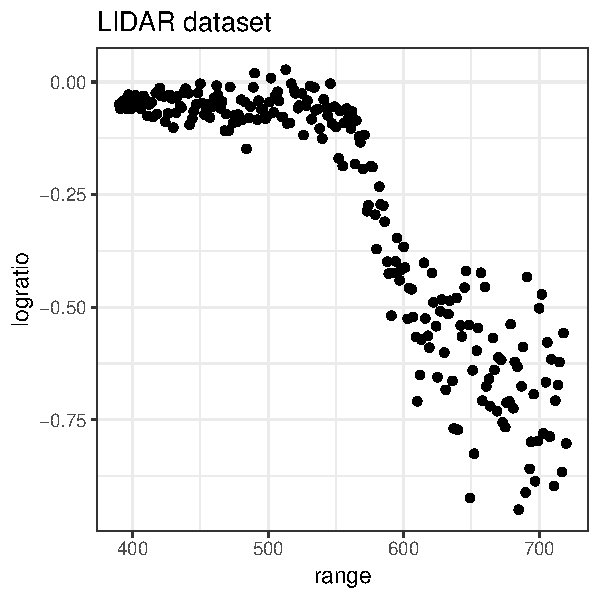
\includegraphics[width=\maxwidth]{figure/lidarPlot-1} 

}



\end{knitrout}
\column{0.58\textwidth}
\small LIDAR = LIght Detection And Ranging
\begin{itemize}
\item it is a surveying method that measures distance to a target by illuminating the target with laser light and measuring the reflected light with a sensor
\item $x$: distance travelled before the light is reflected back to its source
\item $y$: logarithm of the ratio of received light from two laser sources
\end{itemize}
\end{columns}

% \bigskip
\vfill

\uncover<2->{
The objective is to estimate:
$$
f(x) = E \left[ Y \mid X=x \right]
$$
}

\end{frame}




%%%%%%%%%%%%%%%%%%%%%%%%%%%%%%%%%%%%%%%%%%%%%%%%%%%%%%%%%%%%%
\begin{frame}
\frametitle{What does local mean?}
\begin{columns}
\column[t]{0.52\textwidth}
\only<1->{
\small If we had enough points with $x=x_0$

\begin{knitrout}
\definecolor{shadecolor}{rgb}{0.969, 0.969, 0.969}\color{fgcolor}

{\centering 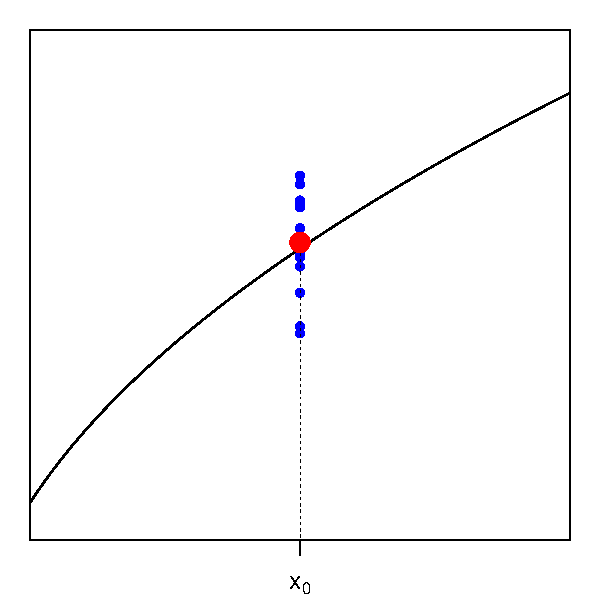
\includegraphics[width=\maxwidth]{figure/local-1} 

}



\end{knitrout}
}
\column[t]{0.52\textwidth}
\only<2->{
\small We can consider points "close" to $x_0$

\begin{knitrout}
\definecolor{shadecolor}{rgb}{0.969, 0.969, 0.969}\color{fgcolor}

{\centering 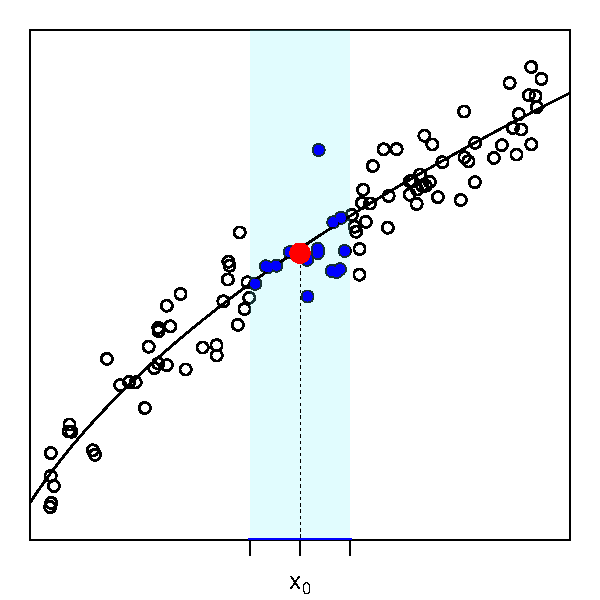
\includegraphics[width=\maxwidth]{figure/neighborhood-1} 

}



\end{knitrout}
}
\end{columns}
\end{frame}

%%%%%%%%%%%%%%%%%%%%%%%%%%%%%%%%%%%%%%%%%%%%%%%%%%%%%%%%%%%%%
\begin{frame}
\frametitle{2 basic ideas}
\begin{columns}
\column[t]{0.52\textwidth}
\begin{block}{$k$ nearest neighbors}
$$ \hat{f}(x) = \frac{1}{k} \sum_{i=1}^n y_i I_{N_k(x)}(x_i) $$

\end{block}
\column[t]{0.52\textwidth}
\begin{block}{Neighborhood of radius $h$}
$$\hat{f}(x) = \frac{\sum_{i=1}^n y_i I_{[0,h]}(|x-x_i|)}{\sum_{i=1}^n I_{[0,h]}(|x-x_i|)}$$

\end{block}
\end{columns}


\begin{columns}
\column[t]{0.52\textwidth}
\begin{knitrout}
\definecolor{shadecolor}{rgb}{0.969, 0.969, 0.969}\color{fgcolor}

{\centering 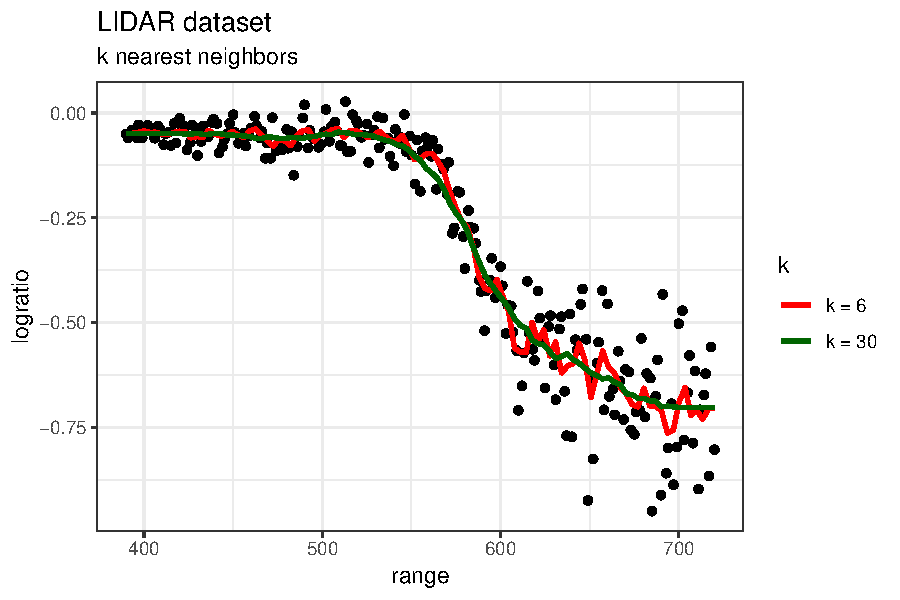
\includegraphics[width=\maxwidth]{figure/lidarKnn-1} 

}



\end{knitrout}
\column[t]{0.52\textwidth}
\begin{knitrout}
\definecolor{shadecolor}{rgb}{0.969, 0.969, 0.969}\color{fgcolor}

{\centering 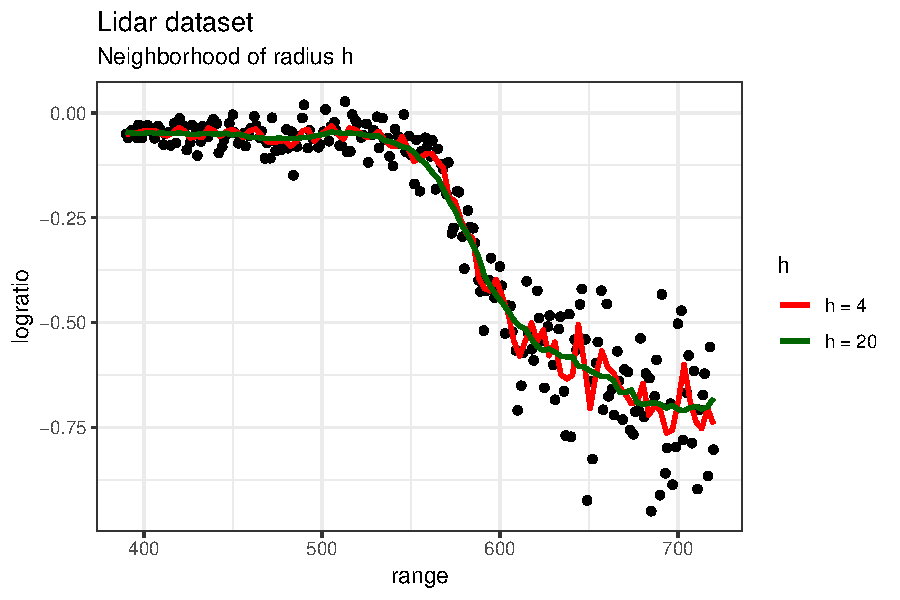
\includegraphics[width=\maxwidth]{figure/lidarRadiusH-1} 

}



\end{knitrout}
\end{columns}
\end{frame}

%%%%%%%%%%%%%%%%%%%%%%%%%%%%%%%%%%%%%%%%%%%%%%%%%%%%%%%%%%%%%
\begin{frame}
\frametitle{Nadaraya-Watson kernel regression}

$$
\hat{f}(x) = \sum_{i=1}^n \ell_i(x) y_i
$$

with:
$$
\ell_i(x) = \frac{K\left(\frac{x-x_i}{h}\right)}{\sum_{j=1}^n K\left(\frac{x-x_j}{h}\right)}
$$

where $K(\cdot)$ is a kernel function that satisfies:
\begin{itemize}
\item $ K(x)\geq 0$
\item $ \int K(x)dx=1$
\item $ \int xK(x)dx=0$
\item $ \int x^2K(x)dx>0$
\end{itemize}


% $$
% I_{[0,h]}(|x-x_i|) = I_{[-1,1]}\left(\frac{x-x_i}{h}\right)
% $$

\end{frame}

%%%%%%%%%%%%%%%%%%%%%%%%%%%%%%%%%%%%%%%%%%%%%%%%%%%%%%%%%%%%%
\begin{frame}
\frametitle{Some proposed kernels}



\resizebox{\textwidth}{!}{
\begin{tabular}{cccc}
Uniform &
\multirow{4}{*}{
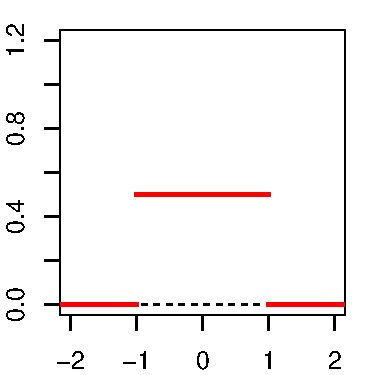
\includegraphics[width=0.18\textwidth]{figure/uniform-1}
}%
& 
Triangle &
\multirow{4}{*}{
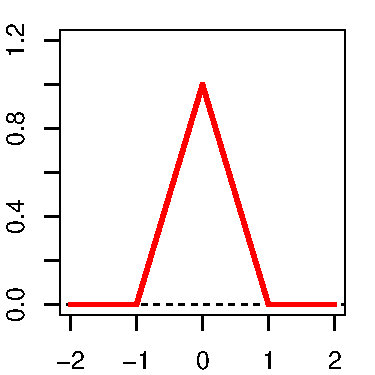
\includegraphics[width=0.18\textwidth]{figure/triangle-1}
}%
\\
$\frac{1}{2}I_{[-1,1]}(u)$ & &  $(1-|u|)I_{[-1,1]}(u)$ & \\ & & & \\ & & & \\
Triweight &
\multirow{4}{*}{
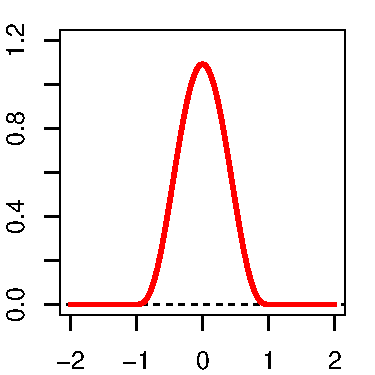
\includegraphics[width=0.18\textwidth]{figure/triweight-1}
}%
& 
Quartic &
\multirow{4}{*}{
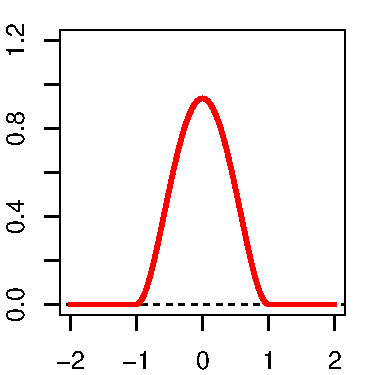
\includegraphics[width=0.18\textwidth]{figure/quartic-1}
}%
\\
 $\frac{35}{32}(1-u^2)^3I_{[-1,1]}(u)$ & &   $\frac{15}{16}(1-u^2)^2I_{[-1,1]}(u)$ & \\ & & & \\ & & & \\
Cosine &
\multirow{4}{*}{
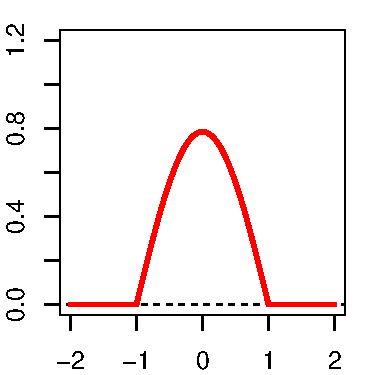
\includegraphics[width=0.18\textwidth]{figure/cosine-1}
}%
& 
Epanechnikov &
\multirow{4}{*}{
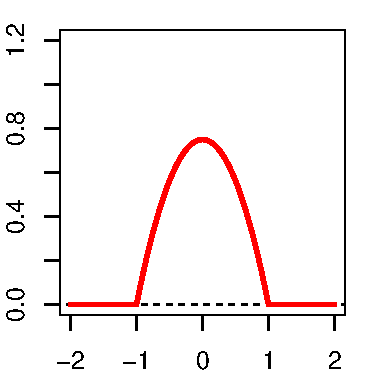
\includegraphics[width=0.18\textwidth]{figure/epanechnikov-1}
}%
\\
$\frac{\pi}{4}\cos\left(\frac{\pi}{2}u\right)I_{[-1,1]}(u)$ & &    $\frac{3}{4}(1-u^2)I_{[-1,1]}(u)$  & \\ & & & \\ & & & \\
Gaussian &
\multirow{4}{*}{
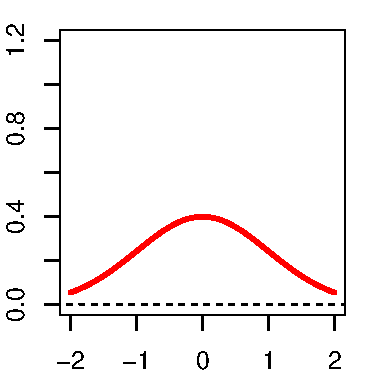
\includegraphics[width=0.18\textwidth]{figure/gaussian-1}
}%
& 
Tricube &
\multirow{4}{*}{
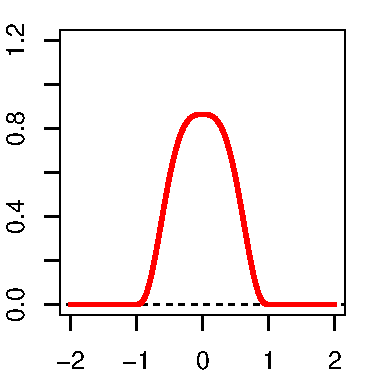
\includegraphics[width=0.18\textwidth]{figure/tricube-1}
}%
\\
$\frac{1}{\sqrt{2\pi}} e^{-u^2/2}$ & & $\frac{70}{81}(1-|u|^3)^3I_{[-1,1]}(u)$ & \\ & & & \\ & & & \\

\end{tabular}
}


\end{frame}

%%%%%%%%%%%%%%%%%%%%%%%%%%%%%%%%%%%%%%%%%%%%%%%%%%%%%%%%%%%%%
\begin{frame}
\frametitle{Design bias, boundary bias and concavity bias}

\begin{knitrout}
\definecolor{shadecolor}{rgb}{0.969, 0.969, 0.969}\color{fgcolor}

{\centering 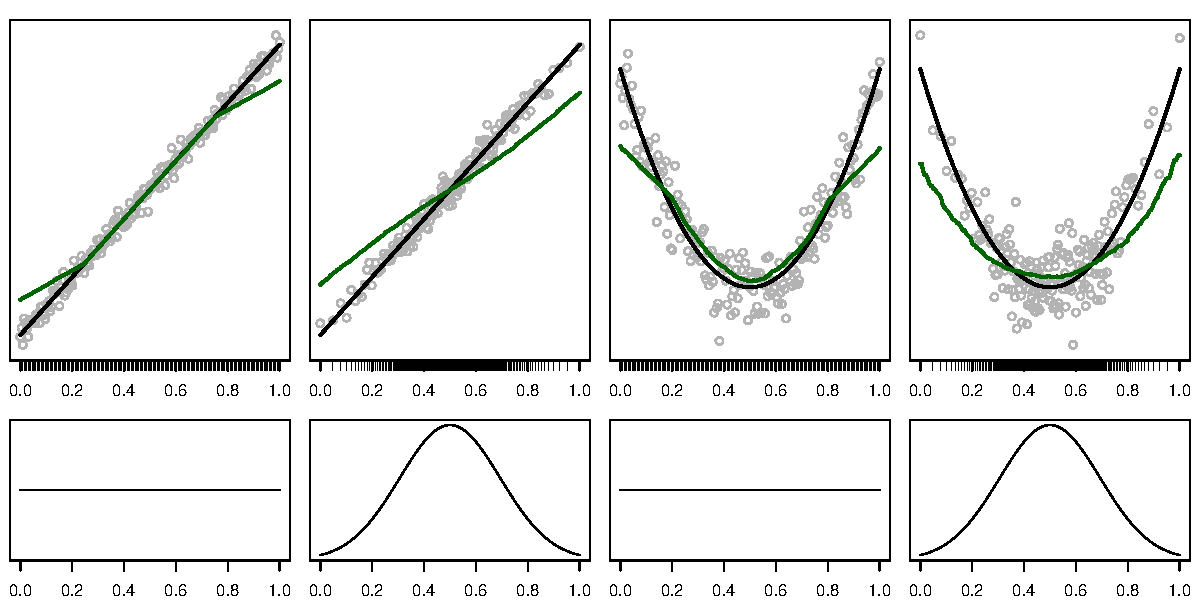
\includegraphics[width=\maxwidth]{figure/nw_bias-1} 

}



\end{knitrout}



\end{frame}

%%%%%%%%%%%%%%%%%%%%%%%%%%%%%%%%%%%%%%%%%%%%%%%%%%%%%%%%%%%%%
\begin{frame}
\frametitle{Design bias: what's happening?}

\begin{knitrout}
\definecolor{shadecolor}{rgb}{0.969, 0.969, 0.969}\color{fgcolor}

{\centering 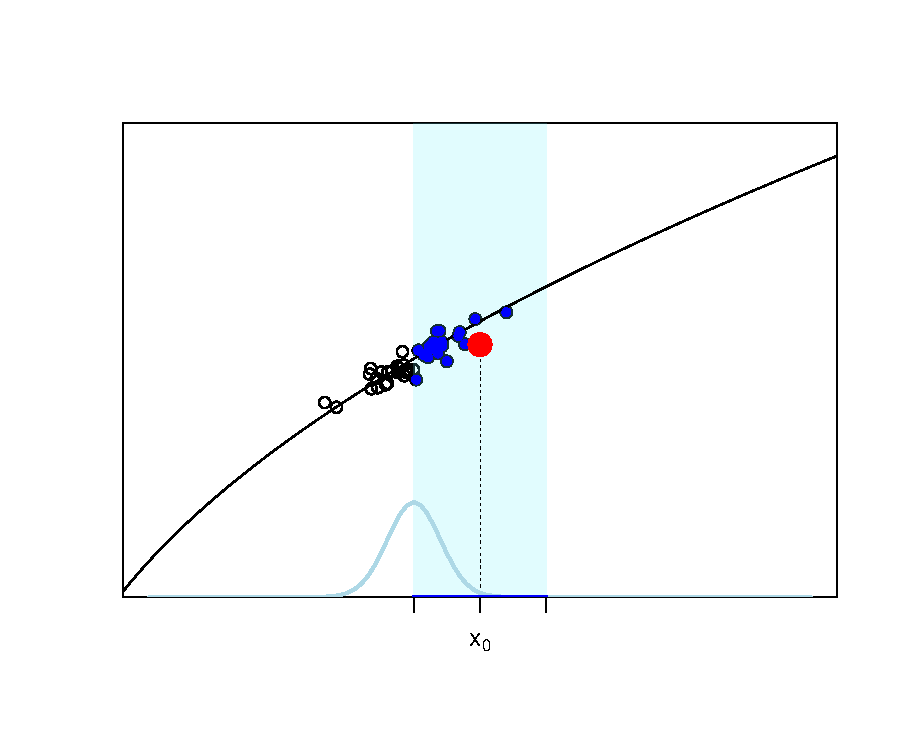
\includegraphics[width=\textwidth]{figure/designBias-1} 

}



\end{knitrout}

\end{frame}



%%%%%%%%%%%%%%%%%%%%%%%%%%%%%%%%%%%%%%%%%%%%%%%%%%%%%%%%%%%%%
\begin{frame}
\frametitle{Local polynomial regression: idea}

Locally the Nadaraya-Watson estimator is a Weighted Least Square Estimator:
$$
\hat{f}_{NW}(x_0) = \underset{a}{\mbox{argmin}} \sum_{i=1}^n K\left(\frac{x_i-x_0}{h}\right)(y_i - a)^2
$$

\hfill

\uncover<2->{
Idea: instead of approximating $f(x_0)$ with a constant value $a$, we could approximate it with a polynomial $p_{x_0}(u, \boldsymbol{a})$.

\hfill

Taylor polynomial approximation:
$$
p_{x_0}(u; \boldsymbol{a}) = a_0 + a_1(u-x_0) + \frac{a_2}{2!}(u-x_0)^2 +\ldots + \frac{a_d}{d!}(u-x_0)^d
$$
}

\end{frame}

%%%%%%%%%%%%%%%%%%%%%%%%%%%%%%%%%%%%%%%%%%%%%%%%%%%%%%%%%%%%%
\begin{frame}
\frametitle{Local polynomial regression: estimation}

We can estimate the coefficients of $p_{x_0}(u;\boldsymbol{a})$ as:
$$
\hat{\boldsymbol{a}}(x_0) = \underset{\boldsymbol{a}}{\mbox{argmin}}
\sum_{i=1}^n K\left(\frac{x_i-x_0}{h}\right)\left(y_i - p_{x_0}(x_i;{\boldsymbol{a}})\right)^2
$$

Thus, we can define the estimator for $f(x)$ in $x_0$ just computing $p_{x_0}(u;\hat{\boldsymbol{a}})$ in $x_0$:

$$
\hat{f}(x_0) = p_{x_0}(x_0; \hat{\boldsymbol{a}})
$$

Then we can repeat the process for each value of $x$ in a grid and obtain $\hat{f}(x)$.

\end{frame}

%%%%%%%%%%%%%%%%%%%%%%%%%%%%%%%%%%%%%%%%%%%%%%%%%%%%%%%%%%%%%
\begin{frame}
\frametitle{Local polynomial regression: example}





\begin{knitrout}
\definecolor{shadecolor}{rgb}{0.969, 0.969, 0.969}\color{fgcolor}

{\centering 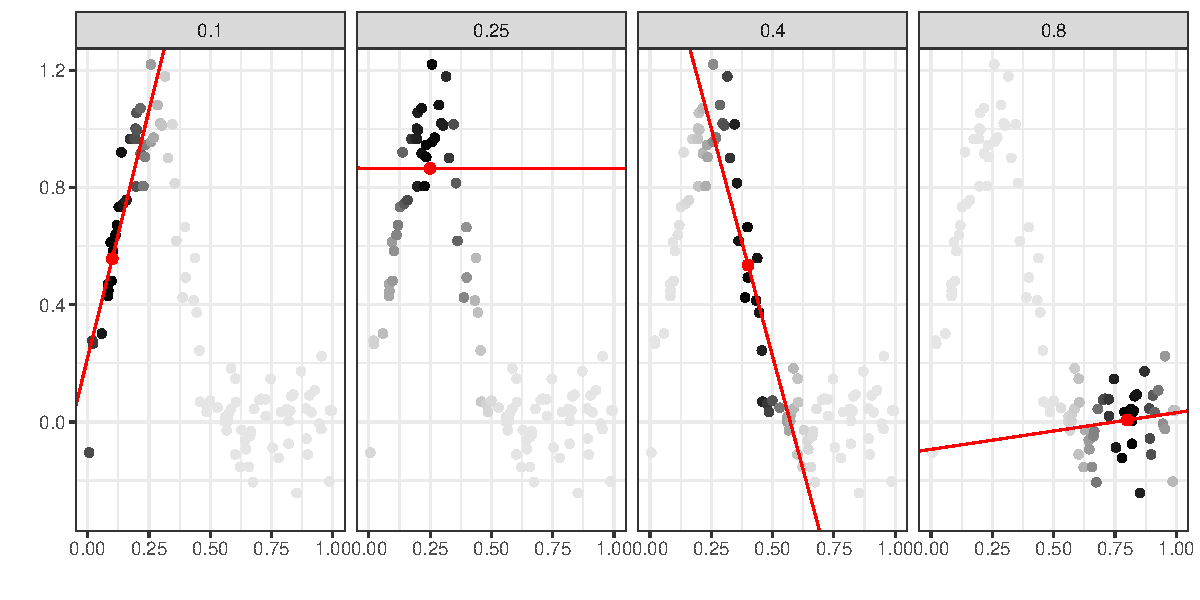
\includegraphics[width=\maxwidth]{figure/LoessExplanation_1-1} 

}



\end{knitrout}



\end{frame}

%%%%%%%%%%%%%%%%%%%%%%%%%%%%%%%%%%%%%%%%%%%%%%%%%%%%%%%%%%%%%
\begin{frame}
\frametitle{Local polynomial regression: example}
\begin{knitrout}
\definecolor{shadecolor}{rgb}{0.969, 0.969, 0.969}\color{fgcolor}

{\centering 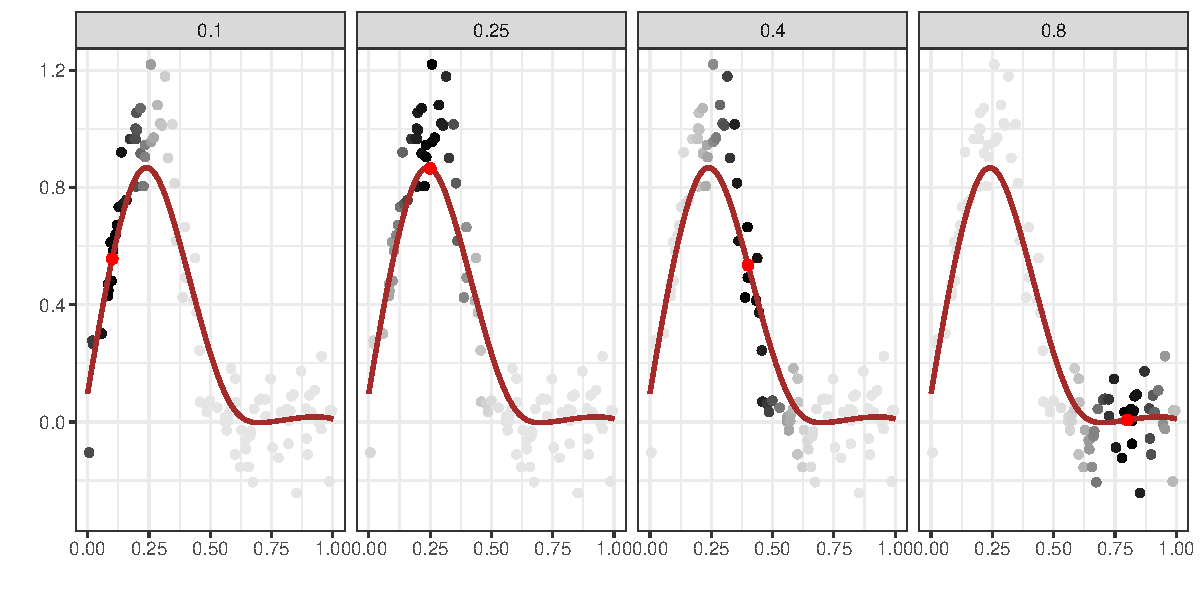
\includegraphics[width=\maxwidth]{figure/LoessExplanation_2-1} 

}



\end{knitrout}
\end{frame}


%%%%%%%%%%%%%%%%%%%%%%%%%%%%%%%%%%%%%%%%%%%%%%%%%%%%%%%%%%%%%
\begin{frame}
\frametitle{Local polynomial regression: example}
\begin{knitrout}
\definecolor{shadecolor}{rgb}{0.969, 0.969, 0.969}\color{fgcolor}

{\centering 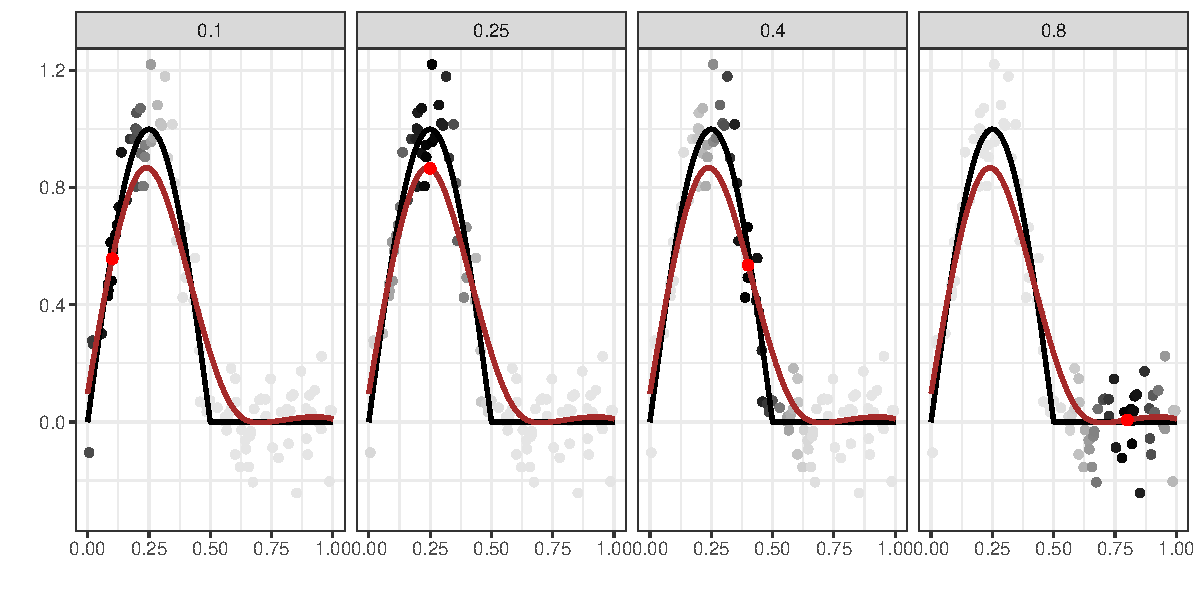
\includegraphics[width=\maxwidth]{figure/LoessExplanation_3-1} 

}



\end{knitrout}

\end{frame}


%%%%%%%%%%%%%%%%%%%%%%%%%%%%%%%%%%%%%%%%%%%%%%%%%%%%%%%%%%%%%
\begin{frame}
\frametitle{Local polynomial regression: example}
\begin{knitrout}
\definecolor{shadecolor}{rgb}{0.969, 0.969, 0.969}\color{fgcolor}

{\centering 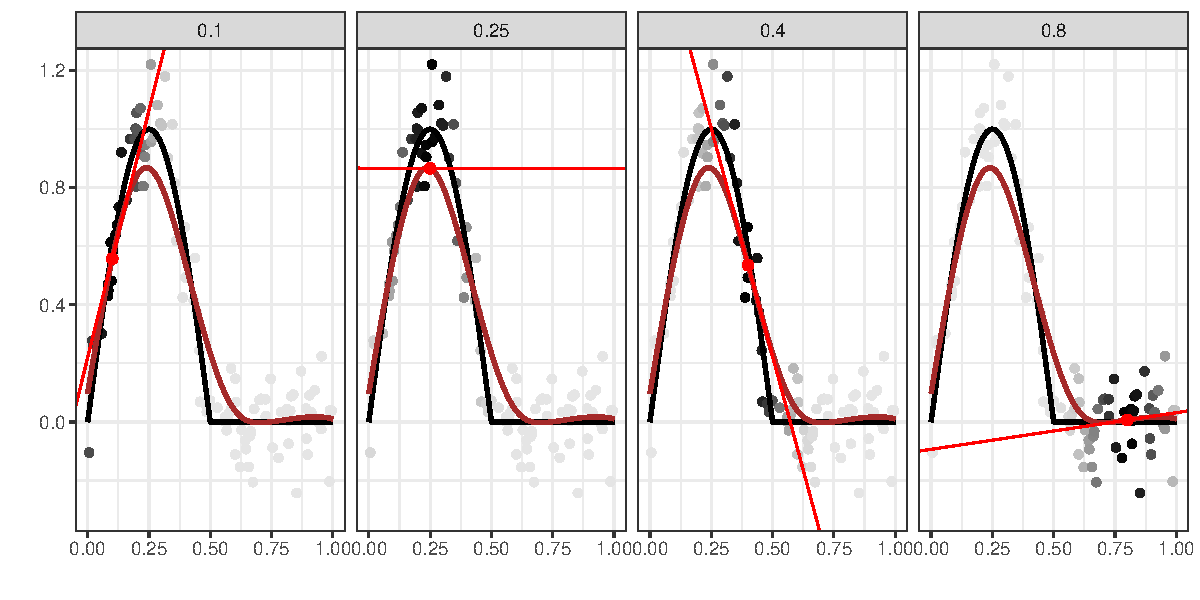
\includegraphics[width=\maxwidth]{figure/LoessExplanation_4-1} 

}



\end{knitrout}

\end{frame}


%%%%%%%%%%%%%%%%%%%%%%%%%%%%%%%%%%%%%%%%%%%%%%%%%%%%%%%%%%%%%
\begin{frame}
\frametitle{Design bias, boundary bias and concavity bias}
\begin{knitrout}
\definecolor{shadecolor}{rgb}{0.969, 0.969, 0.969}\color{fgcolor}

{\centering 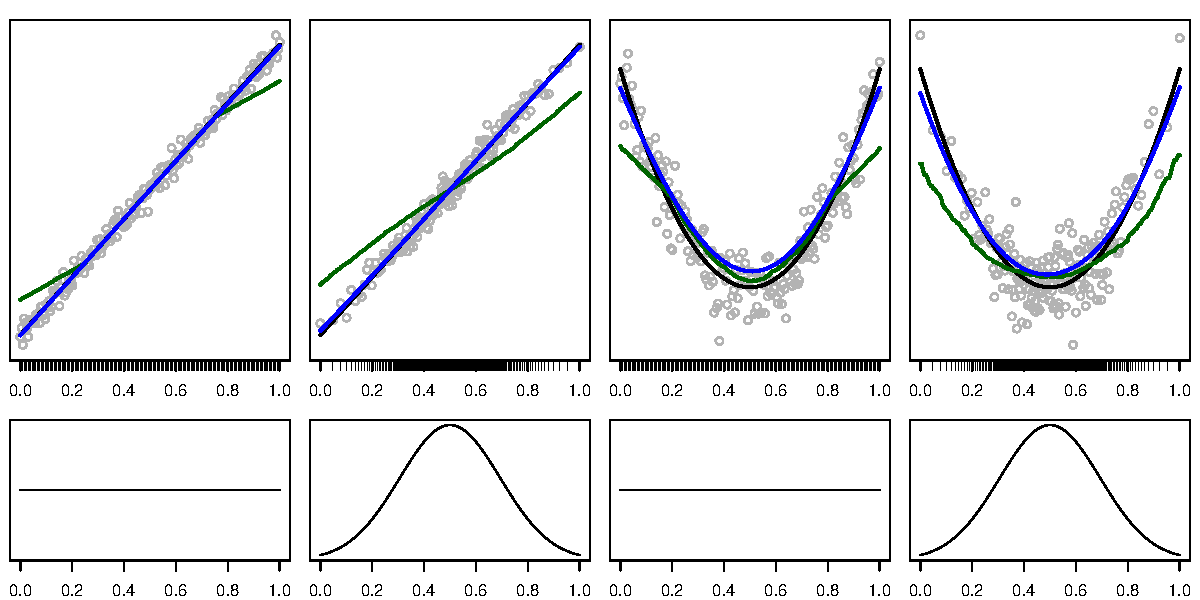
\includegraphics[width=\maxwidth]{figure/loess_bias-1} 

}



\end{knitrout}
\end{frame}


%%%%%%%%%%%%%%%%%%%%%%%%%%%%%%%%%%%%%%%%%%%%%%%%%%%%%%%%%%%%%
\begin{frame}
\frametitle{Local Polynomial Regression on LIDAR dataset}
\begin{knitrout}
\definecolor{shadecolor}{rgb}{0.969, 0.969, 0.969}\color{fgcolor}

{\centering \includegraphics[width=\maxwidth]{figure/lidarLoess-1} 

}



\end{knitrout}
\end{frame}


%%%%%%%%%%%%%%%%%%%%%%%%%%%%%%%%%%%%%%%%%%%%%%%%%%%%%%%%%%%%%
\begin{frame}
\frametitle{Local polynomial regression: linear vs quadratic}

\begin{knitrout}
\definecolor{shadecolor}{rgb}{0.969, 0.969, 0.969}\color{fgcolor}

{\centering 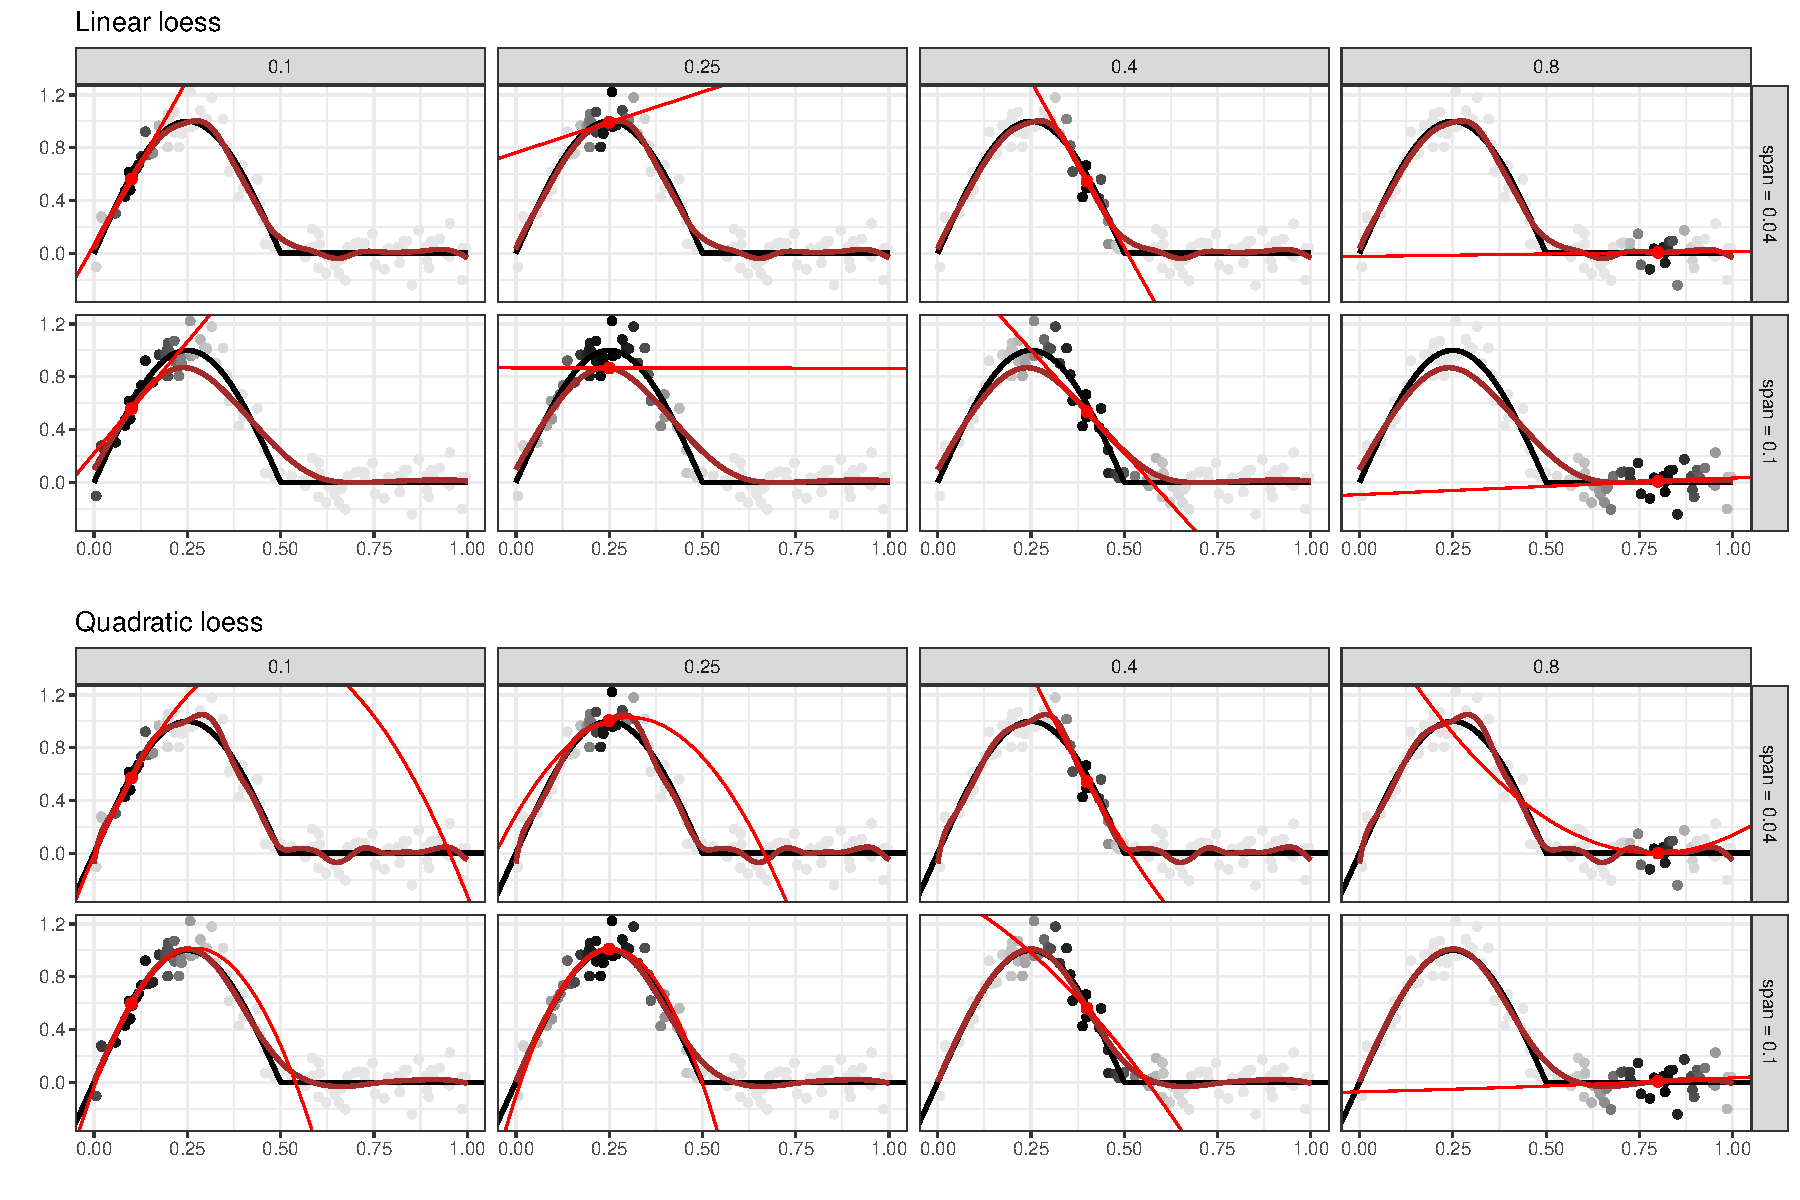
\includegraphics[width=\maxwidth]{figure/LoessComparison-1} 

}



\end{knitrout}

\end{frame}


%%%%%%%%%%%%%%%%%%%%%%%%%%%%%%%%%%%%%%%%%%%%%%%%%%%%%%%%%%%%%
\begin{frame}
\frametitle{Bibliography}

\begin{columns}
\column[t]{0.5\textwidth}
\small
\textbf{Fan, Gijbels} \\
\textit{Local Polynomial Modelling and its Applications} \\
Springer (1996)
\column[t]{0.5\textwidth}
\small
\textbf{Ruppert, Wand, Carroll} \\
\textit{Semiparametric Regression} \\
Cambridge University Press (2003)
\end{columns}

\begin{columns}
\column{0.5\textwidth}
\begin{center}
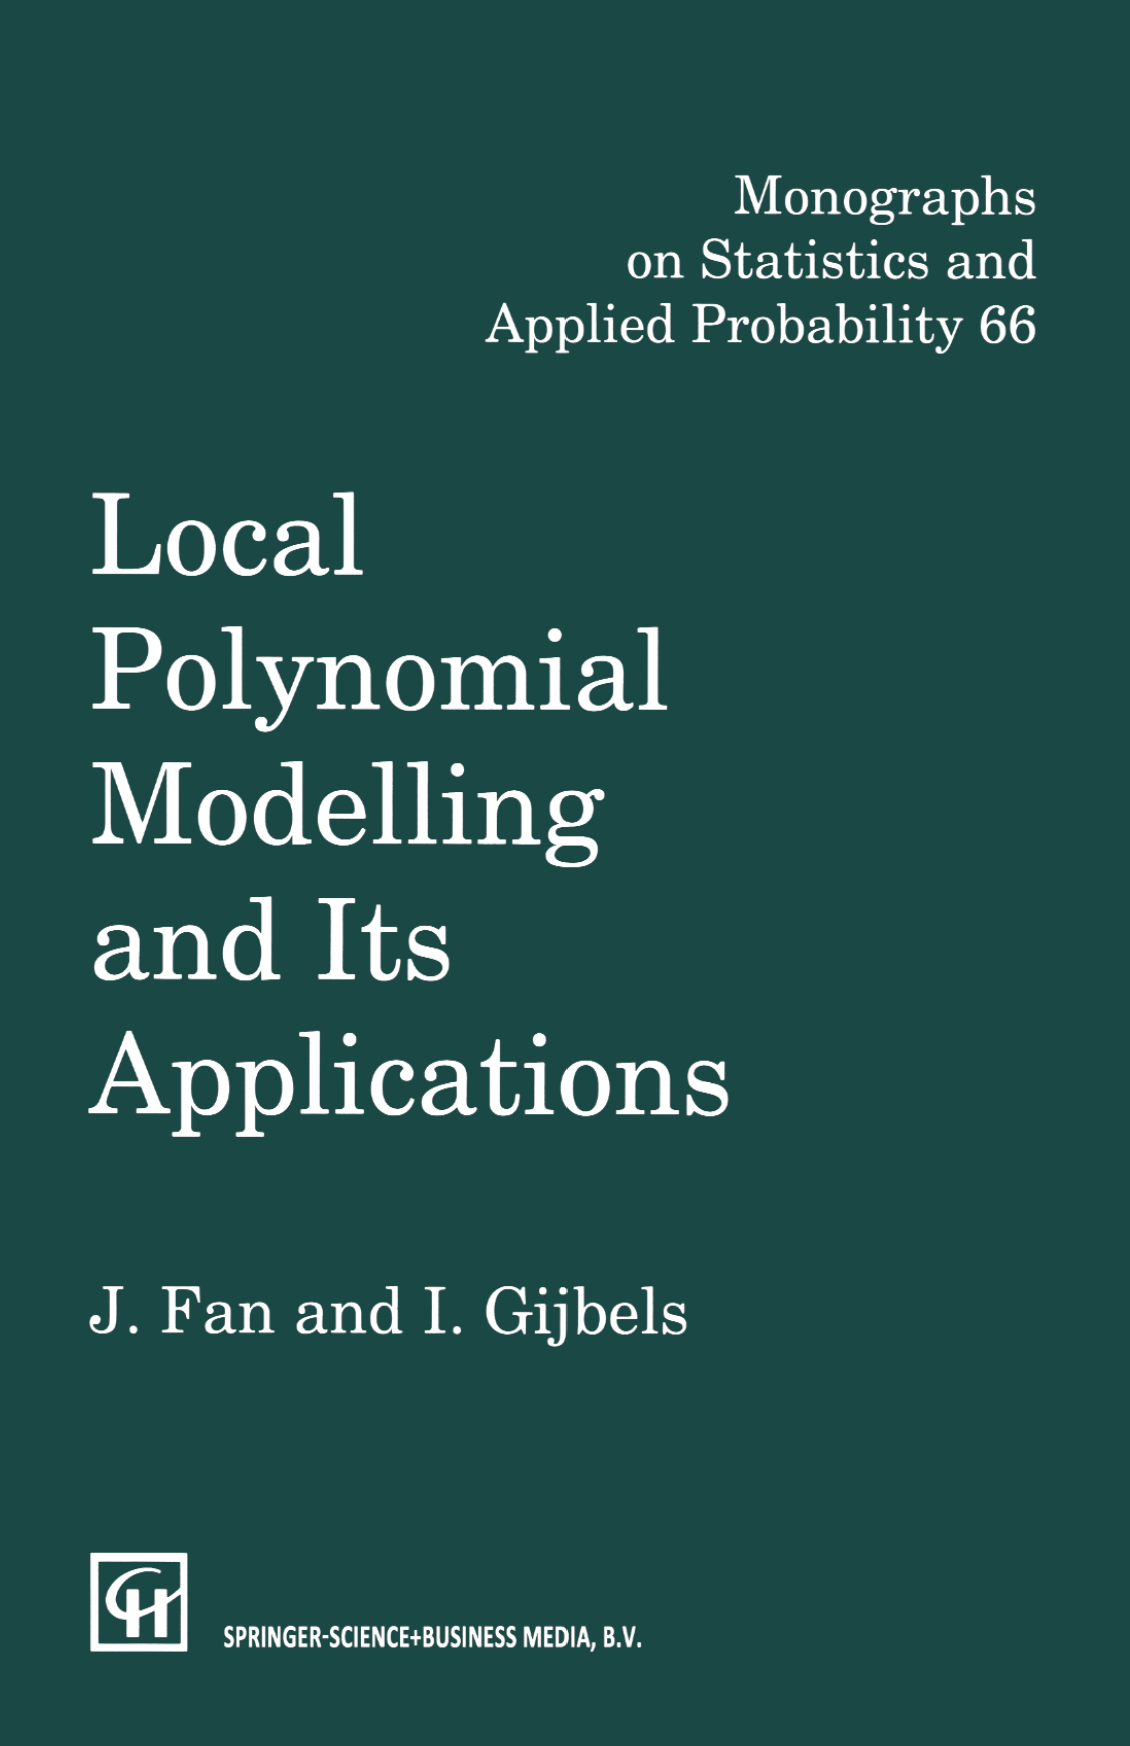
\includegraphics[width=0.6\textwidth]{img/cover_localPolynomialModellingAndItsApplication.png}
\end{center}
\column{0.5\textwidth}
\begin{center}
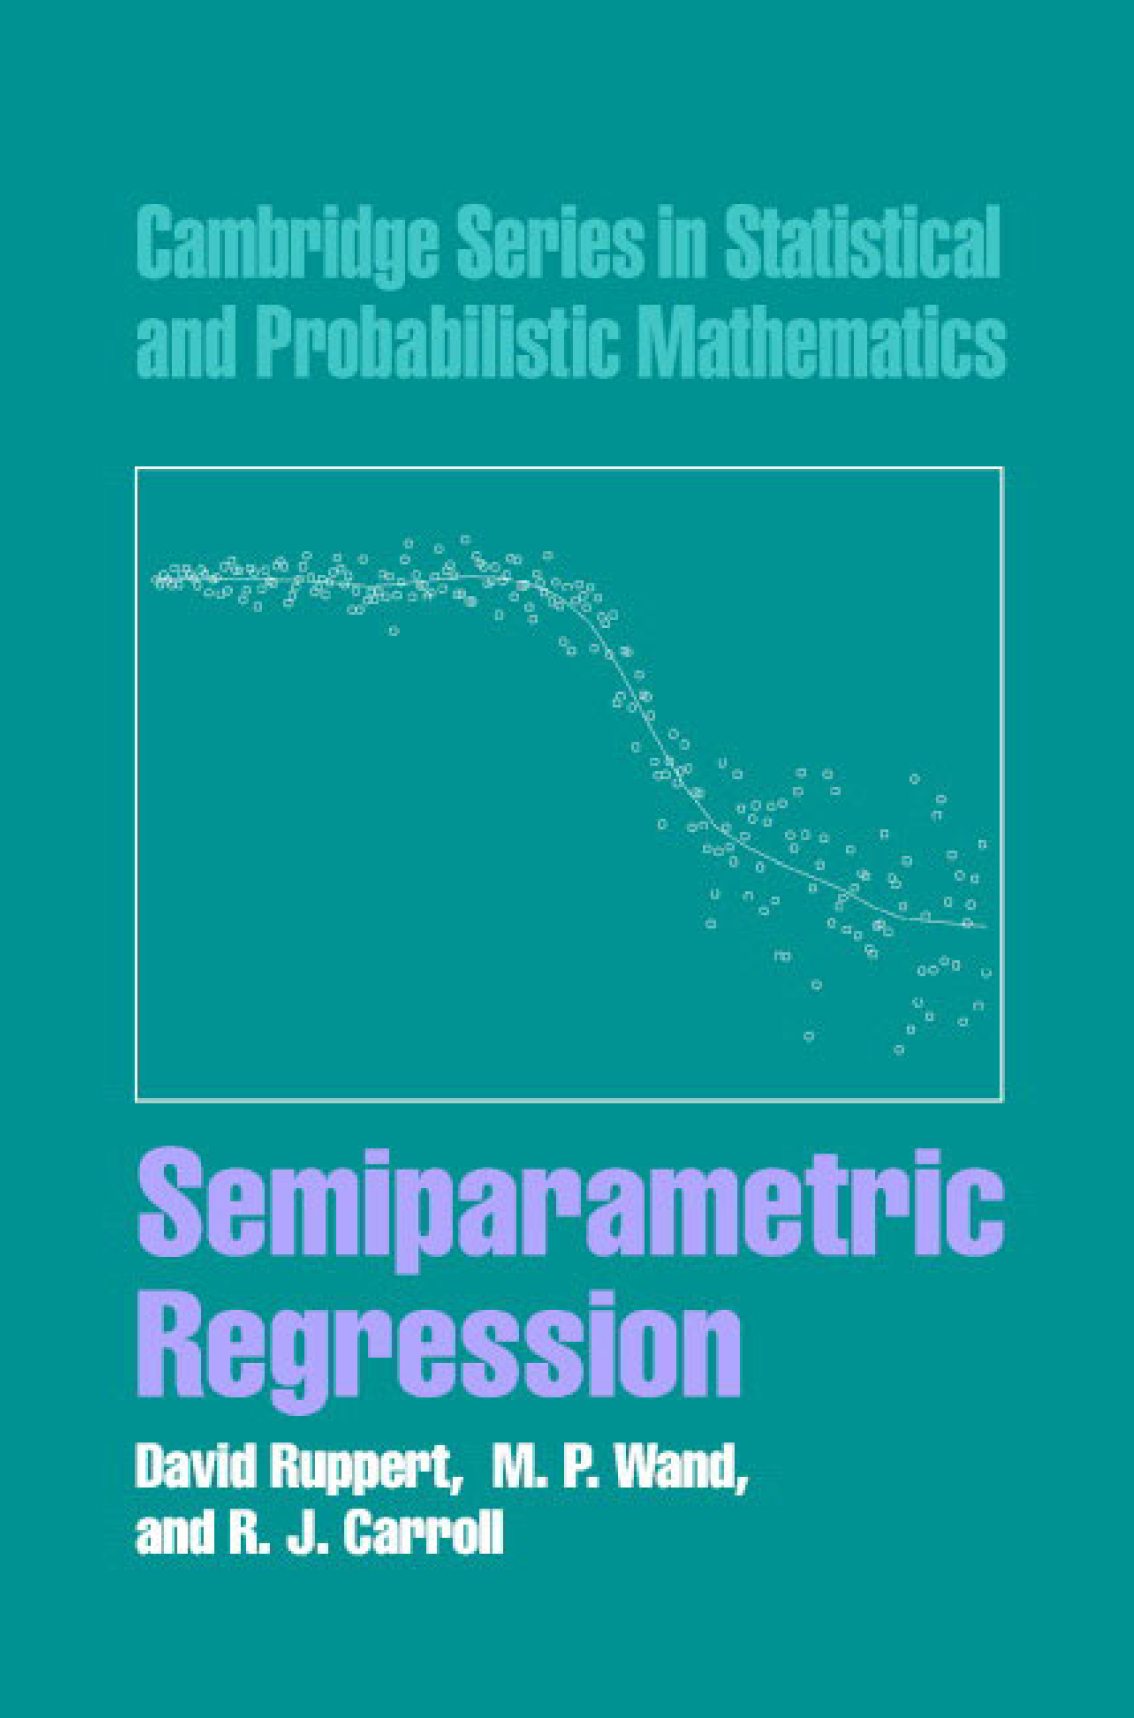
\includegraphics[width=0.6\textwidth]{img/cover_semiparametriRegression.png}
\end{center}
\end{columns}

\end{frame}


\end{document}
